\documentclass[twocolumn,english]{IEEEtran}
\usepackage[T1]{fontenc}
\usepackage{babel}
\usepackage{amsthm}
\usepackage{amsmath}
\usepackage{graphicx}
\usepackage[unicode=true,
 bookmarks=true,bookmarksnumbered=true,bookmarksopen=true,bookmarksopenlevel=1,
 breaklinks=false,pdfborder={0 0 0},backref=false,colorlinks=false]
 {hyperref}
\usepackage{bm}
\usepackage{amsmath}
\usepackage{amssymb}
\usepackage{natbib}
\usepackage{array}
\usepackage{calc}
\newcolumntype{W}{>{\centering\arraybackslash}m{25mm}}
\newcolumntype{L}{>{\centering\arraybackslash}m{15mm}}


\hypersetup{
 pdftitle=  {Lab 6: Electric Power},
 pdfauthor= {Zack Garza},
 pdfpagelayout=OneColumn, pdfnewwindow=true, pdfstartview=XYZ, plainpages=false}

\makeatletter


%%%%%%%%%%%%%%%%%%%%%%%%%%%%%% Textclass specific LaTeX commands.
 % protect \markboth against an old bug reintroduced in babel >= 3.8g
 \let\oldforeign@language\foreign@language
 \DeclareRobustCommand{\foreign@language}[1]{%
   \lowercase{\oldforeign@language{#1}}}
\theoremstyle{plain}
\newtheorem{thm}{\protect\theoremname}
\theoremstyle{plain}
\newtheorem{lem}[thm]{\protect\lemmaname}

%%%%%%%%%%%%%%%%%%%%%%%%%%%%%% User specified LaTeX commands.
% for subfigures/subtables
\ifCLASSOPTIONcompsoc
\usepackage[caption=false,font=normalsize,labelfont=sf,textfont=sf]{subfig}
\else
\usepackage[caption=false,font=footnotesize]{subfig}
\fi

\makeatother
\providecommand{\lemmaname}{Lemma}
\providecommand{\theoremname}{Theorem}
\setcounter{topnumber}{2}
\setcounter{bottomnumber}{2}
\setcounter{totalnumber}{4}
\renewcommand{\topfraction}{0.85}
\renewcommand{\bottomfraction}{0.85}
\renewcommand{\textfraction}{0.15}
\renewcommand{\floatpagefraction}{0.7}
\usepackage{float}
\begin{document}

\title{Electric Power and Impedance Matching}


\author{Zack Garza}


\IEEEspecialpapernotice
{Physics 210L \\
Effective Date of Report: \today}


\markboth{Electric Power}{Zack Garza}
\maketitle
\begin{abstract}
\IEEEPARstart{T}{he} purpose of this experiment is to use Kirchoff's Voltage Law to determine the internal resistance and the open circuit voltage of a power supply by examining the effects of varying load resistances on current and voltage measurements over the load. These measurements will also be used to determine the resistance at which maximum power is delivered to a load via impedance matching.
\end{abstract}
\tableofcontents

\section{Theory}
\begin{figure}[h!]
  \begin{centering}
  \begin{center}
  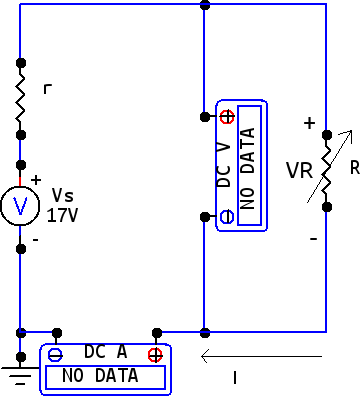
\includegraphics[width=\linewidth]{./Images/circuit.png}
  \caption{Diagram of circuit used in this experiment. $R$ represents a variable load resistance, while $r$ simulates the internal resistance of the power supply. $I$ is the uniform current that flows through all three components of the circuit.}
  \label{fig:circuit_diagram}
  \end{center}
  \par\end{centering}
  \end{figure}

\textbf{Kirchoff's Voltage Law} states that the sum of the potential differences in a closed loop is equal to zero, such that
\begin{equation*}
 \sum V_{\text{Loop}} = 0.
\end{equation*}

For the circuit shown, the potential difference $V_R$ across the load resistor can be found using this equation. Summing the voltages and rewriting them using $V=iR$ (according to Ohm's Law) yields
\begin{align}\label{eq:part1}
 \epsilon - V_{r} - V_R &= 0 	\Rightarrow \notag \\
 V_R &= \epsilon - V_r 		\Rightarrow \notag \\
 V_R &= \epsilon - ir
\end{align}
where the current $i$ is identical throughout the circuit, as its elements are wired in series, and $r$ is the power supply's internal voltage.

The power released by the resistor $R$ can also be expressed in terms of the known quantities $\epsilon, r$, and $R$. From the power equation, it is known that $P=iV$. Because the current $i$ is uniform everywhere, it can be related to the source voltage and the equivalent resistance of the entire circuit. Taking the source voltage to as $\epsilon$ and the equivalent resistance as $r+R$ and substituting it into the power equation yields
\begin{align}\label{eq:part2}
 P = iV, V = iR \Rightarrow P = \frac{i^2}{R} 	\Rightarrow \notag 	\\
 P_R = \left(\frac{\epsilon}{r+R}\right)^2 R 	\Rightarrow \notag	\\
 P_R = \epsilon^2 \frac{R}{(r+R)^2}.
\end{align}

Calculating the point at which maximum power transfer occurs requires taking the derivative of Equation~\ref{eq:part2} with respect to the load resistance. This results in
\begin{align*}
 \frac{\partial P}{\partial R} = \epsilon^2 \left(\frac{(r+R^2)-2R(R+r)}{(R+r)^4}\right).
\end{align*}

Maximizing the power transferred to the load resistor requires setting this derivative equal to zero, which occurs when
\begin{align*}
 r+R^2 = 2R(R+r).
\end{align*}

Solving this expression for $R$ then forces the following condition to be true in order to maximize the power delivered to the load resistor $R$:
\begin{align}
 R=r.
\end{align}

\section{Methodology}
\begin{enumerate}
 \item The circuit was constructed as shown in Figure~\ref{fig:circuit_diagram}, where $r$ was a known resistor and $R$ was a variable resistor box.
 \item Digital voltmeters and ammeters were wired to measure $V_R$ and $i$.
 \item The power supply was set to 17.00 V, and its actual terminal voltage was measured.
 \item The known resistor $r$ was measured with an ohmmeter.
 \item The resistance of the variable load was incremented, and at each point data was taken for the voltage and current through $R$.
 \item Extra data points were taken at resistances approaching that of the known resistor.
\end{enumerate}

\noindent \hrulefill

\section{Data}
\begin{table}[htpb]
\centering
\caption{Circuit measurements and calculated values.}\label{tb:data}
\begin{tabular}{|l|l|l|l|l|}
\hline
\multicolumn{1}{|c}{\textbf{\begin{tabular}[c]{@{}c@{}}Box Setting\\ R ($\Omega$)\end{tabular}}} & \multicolumn{1}{|c}{\textbf{\begin{tabular}[c]{@{}c@{}}Voltage\\ (V)\end{tabular}}} & \multicolumn{1}{|c}{\textbf{\begin{tabular}[c]{@{}c@{}}Current\\ (mA)\end{tabular}}} & \multicolumn{1}{|c}{\textbf{\begin{tabular}[c]{@{}c@{}}$R_{\text{Calc}}$\\ ($\Omega$)\end{tabular}}} & \multicolumn{1}{|c|}{\textbf{Power (W)}} \\ \hline
0                                                                                                & 0.004                                                                               & 30.24                                                                                & 0.13                                                                                                 & 0.00012                              \\ \hline
10                                                                                               & 0.3014                                                                              & 29.69                                                                                & 10.15                                                                                                & 0.00895                              \\ \hline
20                                                                                               & 0.574                                                                               & 28.45                                                                                & 20.18                                                                                                & 0.01633                              \\ \hline
30                                                                                               & 0.845                                                                               & 28.00                                                                                & 30.18                                                                                                & 0.02366                              \\ \hline
40                                                                                               & 1.108                                                                               & 27.60                                                                                & 40.14                                                                                                & 0.03058                              \\ \hline
50                                                                                               & 1.365                                                                               & 27.19                                                                                & 50.20                                                                                                & 0.03711                              \\ \hline
100                                                                                              & 2.531                                                                               & 25.25                                                                                & 100.24                                                                                               & 0.06391                              \\ \hline
200                                                                                              & 4.41                                                                                & 22.03                                                                                & 200.18                                                                                               & 0.09715                              \\ \hline
250                                                                                              & 5.18                                                                                & 20.69                                                                                & 250.36                                                                                               & 0.10717                              \\ \hline
300                                                                                              & 5.86                                                                                & 19.50                                                                                & 300.51                                                                                               & 0.11427                              \\ \hline
350                                                                                              & 6.46                                                                                & 18.44                                                                                & 350.33                                                                                               & 0.11912                              \\ \hline
400                                                                                              & 7.00                                                                                & 17.50                                                                                & 400.00                                                                                               & 0.12250                              \\ \hline
450                                                                                              & 7.50                                                                                & 16.67                                                                                & 449.91                                                                                               & 0.12503                              \\ \hline
475                                                                                              & 7.72                                                                                & 16.24                                                                                & 475.37                                                                                               & 0.12537                              \\ \hline
500                                                                                              & 7.94                                                                                & 15.86                                                                                & 500.63                                                                                               & 0.12593                              \\ \hline
510                                                                                              & 8.02                                                                                & 15.72                                                                                & 510.18                                                                                               & 0.12607                              \\ \hline
520                                                                                              & 8.11                                                                                & 15.57                                                                                & 520.87                                                                                               & 0.12627                              \\ \hline
530                                                                                              & 8.19                                                                                & 15.43                                                                                & 530.78                                                                                               & 0.12637                              \\ \hline
540                                                                                              & 8.27                                                                                & 15.29                                                                                & 540.88                                                                                               & 0.12645                              \\ \hline
545                                                                                              & 8.30                                                                                & 15.22                                                                                & 545.34                                                                                               & 0.12633                              \\ \hline
550                                                                                              & 8.34                                                                                & 15.15                                                                                & 550.50                                                                                               & 0.12635                              \\ \hline
555                                                                                              & 8.38                                                                                & 15.09                                                                                & 555.33                                                                                               & 0.12645                              \\ \hline
560                                                                                              & 8.42                                                                                & 15.02                                                                                & 560.59                                                                                               & 0.12647                              \\ \hline
570                                                                                              & 8.50                                                                                & 14.89                                                                                & 570.85                                                                                               & 0.12657                              \\ \hline
580                                                                                              & 8.57                                                                                & 14.76                                                                                & 580.62                                                                                               & 0.12649                              \\ \hline
590                                                                                              & 8.64                                                                                & 14.63                                                                                & 590.57                                                                                               & 0.12640                              \\ \hline
600                                                                                              & 8.71                                                                                & 14.51                                                                                & 600.28                                                                                               & 0.12638                              \\ \hline
700                                                                                              & 9.37                                                                                & 13.37                                                                                & 700.82                                                                                               & 0.12528                              \\ \hline
800                                                                                              & 9.93                                                                                & 12.39                                                                                & 801.45                                                                                               & 0.12303                              \\ \hline
850                                                                                              & 10.17                                                                               & 11.95                                                                                & 851.05                                                                                               & 0.12153                              \\ \hline
875                                                                                              & 10.29                                                                               & 11.74                                                                                & 876.49                                                                                               & 0.12080                              \\ \hline
900                                                                                              & 10.40                                                                               & 11.55                                                                                & 900.43                                                                                               & 0.12012                              \\ \hline
950                                                                                              & 10.62                                                                               & 11.17                                                                                & 950.76                                                                                               & 0.11863                              \\ \hline
975                                                                                              & 10.73                                                                               & 10.99                                                                                & 976.34                                                                                               & 0.11792                              \\ \hline
1000                                                                                             & 10.82                                                                               & 10.81                                                                                & 1000.93                                                                                              & 0.11696                              \\ \hline
\end{tabular}
\end{table}


\begin{align*}
 r &= \text{\underline{0.549 k$\Omega$}} \\
 \epsilon_{\text{Meas}} &= \text{\underline{17.02 V}}
\end{align*}

  \subsection{\textbf{Linear Fit of $V_R$ vs. $i$}}

  \begin{figure}[htpb]
  \begin{centering}
  \begin{center}
  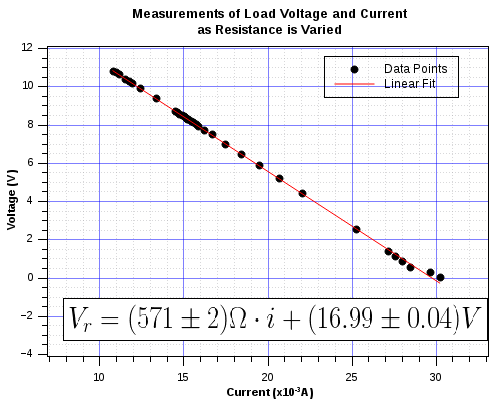
\includegraphics[width=\linewidth]{./Images/vi_graph.png}
  \label{fig:vigraph}
  \caption{Plot of $V_R$ vs. $i$ for the load resistor $R$.}
  \end{center}
  \par\end{centering}
  \end{figure}

  \begin{align*}
   \text{Internal Resistance $r$} 		&=\text{\underline{$(571 \pm 2)\Omega$}}	\\
   \text{Source EMF }\mu_{\text{Theory}}	&=\text{\underline{$(16.99 \pm .04)$V}}
  \end{align*}

  \begin{align*}
   \text{\% Difference in }\epsilon 	&=\text{\underline{0.2\%}}	\\
   \text{\% Difference in }r		&=\text{\underline{3.9\%}}
  \end{align*}

  \subsection{\textbf{Polynomial Fit of $P_R$ vs. $R_{\text{Calc}}$}}

  \begin{figure}[htpb]
  \begin{centering}
  \begin{center}
  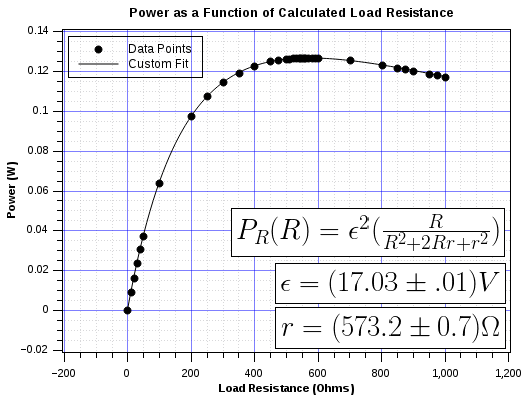
\includegraphics[width=\linewidth]{./Images/power_graph.png}
  \caption{Plot of power (from $P=iV$) vs. Calculated Load Resistance (from $R=\frac{V_R}{i}$), fitted to the expression given in Equation~\ref{eq:part2}.}
  \label{fig:power_graph}
  \end{center}
  \par\end{centering}
  \end{figure}

  \begin{figure}[htpb]
  \begin{centering}
  \begin{center}
  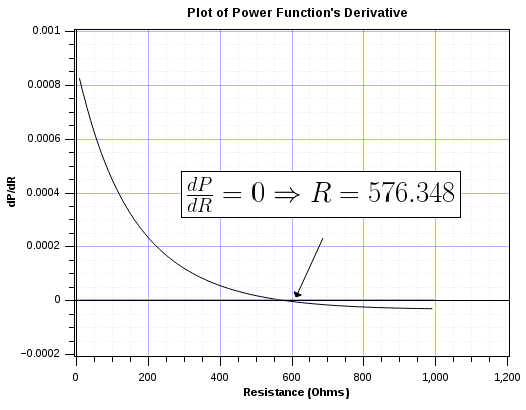
\includegraphics[width=\linewidth]{./Images/power_derivative.png}
  \caption{Plot of the derivative of $P$ vs. $R_{\text{Calculated}}$ and its intersection with 0, giving the resistance at which the maximum power is delivered.}
  \label{fig:power_derivative}
  \end{center}
  \par\end{centering}
  \end{figure}

  \begin{align*}
   r 				&= \text{\underline{$(573.2 \pm 0.7)\Omega$}}	\\
   \text{\% Difference} 	&= \text{\underline{0.38\%}}
  \end{align*}

  \noindent \hrulefill


\section{Analysis}
\begin{enumerate}
 \item
 \textit{How does the resistance box value compare with $R_{\text{Calculated}}$ as the current in the circuit increases?}

  The deviation between the resistance box value and the calculated resistance remains relatively constant, regardless of the current in the circuit. This represents a source of systematic error in this experiment on the order of approximately 1 $\Omega$. In many cases, the calculated value is within .15 $\Omega$ of the box value, which is equal to the amount of resistance that is calculated be in the box when it is set to zero ohms. It is possible that this represents a certain amount of internal resistance in the box's wiring that is added to the value read from the dials.

 \item \textit{How can you determine the value for $R_{\text{Calculated}}$ that gives $P_{\text{R-Max}}$?}

 Equation~\ref{eq:part2} shows that the maximum power will be delivered to the resistor $R$ when its resistance is equal to the internal resistance $r$. Since $r$ was measured to be .549 k$\Omega$, more data points were collected in the 500-600 $\Omega$ range.

 \item \textit{What are the possible discrepancies between the values of $r$ obtained from the two function fits?}

 The first value is derived from measured quantities, which introduces a certain amount of uncertainty from the measurements and from the curve fit itself. The second value is given by a function that is taken from two derived values, which introduces rounding error. It is also fit to a non-linear function, which tends to be more difficult to model accurately. This in turn produces a slightly different value for $r$.

\end{enumerate}


\appendices{}

%\bibliographystyle{plain}
%\bibliography{physbib}

\end{document}